\begin{frame}{PRUNING}
    \begin{figure}
        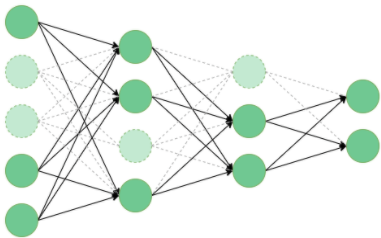
\includegraphics[width = 0.5\linewidth]{pruning no name.png}
    \end{figure}
    Mediante un indice di {\bfseries{\emph{sparsità}}}, è in grado di azzerare e rimuovere (teoricamente) determinati elementi presenti nella rete.
    Il modello su cui è stata applicata tale tecnica è il \emph{Single-Shot-Detector (SSD)}.
    Esistono tre tipi di pruning:
    \begin{enumerate}
        \item {\bfseries{\emph{Structured}}}: rimuove interi filtri (canali);
        \item {\bfseries{\emph{Unstructured}}}: rimuove i parametri (es: pesi e bias) in un layer;
        \item {\bfseries{\emph{Global-Unstructured}}}: rimuove i parametri su più layer.
    \end{enumerate}
    Il framework utilizzato, avente già le API dedicate, è PyTorch.
\end{frame}